% Copyright (C) 2007 Technical University of Liberec.  All rights reserved.
%
% Please make a following reference to Flow123d on your project site if you use the program for any purpose,
% especially for academic research:
% Flow123d, Research Centre: Advanced Remedial Technologies, Technical University of Liberec, Czech Republic
%
% This program is free software; you can redistribute it and/or modify it under the terms
% of the GNU General Public License version 3 as published by the Free Software Foundation.
%
% This program is distributed in the hope that it will be useful, but WITHOUT ANY WARRANTY;
% without even the implied warranty of MERCHANTABILITY or FITNESS FOR A PARTICULAR PURPOSE.
% See the GNU General Public License for more details.
%
% You should have received a copy of the GNU General Public License along with this program; if not,
% write to the Free Software Foundation, Inc., 59 Temple Place - Suite 330, Boston, MA 021110-1307, USA.
%
%%%%%%%%%%%%%%%%%%%%%%%%%%%%%%%%%%%%%%%%%%%%%%%%%%%%%%%%%%%%%%%%%%
%
% use PDFLatex to compile this
%

\documentclass[a4paper]{article}
\usepackage{authblk}
%\usepackage{rotating}
%\usepackage{pdflscape}

\usepackage[bbgreekl]{mathbbol}
\usepackage{amssymb, amsmath, amsthm, stmaryrd}
\newtheorem{theorem}{Theorem}

\usepackage{array}
\usepackage{longtable}
\usepackage[usenames,dvipsnames]{color}   %colors
%\usepackage{colortbl}   %colorful tables
\usepackage{tabularx,tikz}
\usepackage{graphicx} %[dvips]
% it is note used \usepackage{cooltooltips}

%these two can be found in caption package
%\usepackage{caption}
%\usepackage{subcaption}

\usepackage[numbers]{natbib}
\usepackage{ulem}
\usepackage{etoolbox}
\usetikzlibrary{arrows,matrix}


%%%%%%%%%%%%%%%%%%%%%%%%%%%%%%%%%%%%%%%%%%%%%%%%%%%%%%%%%%%%%%%%%%%%%%%%%%%%
% macro for units 
% \def\UNIT#1#2{\ifstrempty{#2}{}{%
% \ifstrequal{#2}{1}{\mathrm{#1}}{\mathrm{#1}^{#2}}%
% }}
% \def\units#1#2#3{\ifstrempty{#1#2#3}{$[-]$}{$[ \UNIT{kg}{#1}\UNIT{m}{#2}\UNIT{s}{#3} ]$}}       %with brackets
% \def\unitss#1#2#3{\ifstrempty{#1#2#3}{$-$}{$ \UNIT{kg}{#1}\UNIT{m}{#2}\UNIT{s}{#3} $}}  %without brackets

\newtheorem{corollary}[theorem]{Corollary}
\newtheorem{lemma}[theorem]{Lemma}

%%%%%%%%%%%%%%%%%%%% specific math macros
\def\abs#1{\lvert#1\rvert}
\def\Abs#1{\bigl\lvert#1\bigr\rvert}
\def\aep{\tilde\ep}
\def\agrad{\tilde\nabla}
\def\avg#1{\left\{\mskip-5mu\left\{#1\right\}\mskip-5mu\right\}}
\def\d {\,{\rm d}}
\def\dist{\operatorname{dist}}
\def\div{\operatorname{div}}
\def\dn{\d\nnu}
\def\dt{\prtl_t}
\def\dual#1#2{\left\langle #1,#2\right\rangle}
\def\ep{\vc\varepsilon}
\def\FF{\vc F}
\def\ff{\vc f}
\def\grad{\nabla}
\def\Hel{\mathcal H}
\def\jmp#1{\left\llbracket #1 \right\rrbracket}
\def\Lapl{\Delta}
\def\Natural{\mathbf N}
\def\nn{\vc n}
\def\nnu{\vc\nu}
\def\norm#1{\|#1\|}
\def\ol{\overline}
\def\pbar{\overline p}
\def\pphi{{\varphi}}
\def\prtl{\partial}
\def\qq{\vc q}
\def\Real{{\mathbf R}}
\def\tn#1{{\mathbb{#1}}}    % tensor
\def\tr{\operatorname{tr}}
\def\tt{\vc t}
\def\U{\vc U}
\def\ubar{\overline\uu}
\def\ul{\underline}
\def\uu{\vc u}
\def\V{\vc V}
\def\Vel{{\mathcal V}} % Sobolev space for elasticity
\def\vc#1{\mathbf{\boldsymbol{#1}}}     % vector
\def\vv{\vc v}
\def\weakly{\rightharpoonup}
\def\xx{\vc x}
\def\yy{{\vc y}}

\newcommand{\eq}[1]{\begin{equation}#1\end{equation}}
\newcommand{\ml}[1]{\begin{multline}#1\end{multline}}
\newcommand{\mls}[1]{\begin{multline*}#1\end{multline*}}

\newcommand{\note}[2]{{\color{blue} \textbf{ #1:} \textit{#2}}}
%% ini_table members
%%%%%%%%%%%%%%%%%%%% specific math macros

\newcommand{\opm}{ % plus and minus in circle
  {\mathbin{
    \mathchoice
      {\buildcirclepm{\displaystyle     }{0.14ex}{0.95}{0.05ex}{.7}}
      {\buildcirclepm{\textstyle        }{0.14ex}{0.95}{0.05ex}{.7}}
      {\buildcirclepm{\scriptstyle      }{0.13ex}{0.955}{0.04ex}{.55}}
      {\buildcirclepm{\scriptscriptstyle}{0.08ex}{0.95}{0.03ex}{.45}}
  }} 
}
\newcommand\buildcirclepm[5]{%
  \begin{tikzpicture}[baseline=(X.base), inner sep=-#5, outer sep=-.65]
    \node[draw,circle,line width=#4] (X)  {\footnotesize\raisebox{#2}{\scalebox{#3}{$#1\pm$}}};
  \end{tikzpicture}%
}


%%%%%%%%%%%%%%%%%%%%%%%%%%%%%%%%%%%%%%%%%%%%%%%%%%%%%%%%%%%%%%%%%%%%%%%%%%%%%%%%%%%%%%%%%%%%% BEGIN DOCUMENT
\begin{document}

\title{Mixed-dimensional models of linear elasticity and poroelasticity}
\author{Jan Březina}
\author{Jan Stebel}
\affil{Technical University of Liberec,\\ Studentská 1402/2, 461 17 Liberec, Czech Republic}
\affil{e-mail: \texttt{\{jan.brezina,jan.stebel\}@tul.cz}}
\maketitle


\section{Introduction}

In this paper we describe a dimension reduction for the Biot system of poroelasticity in a domain containing a fracture, which is assumed to be a thin manifold around a subset of hyperplane.
The obtained equations (eq. \eqref{eq:lin_el_frac}, \eqref{eq:flow_frac}) are expressed in terms of mean pressure and mean displacement in the fracture.
The resulting problem consists of equations of flow and mechanics in the fracture and in the surrounding domain, accompanied by appropriate interface conditions (eq. \eqref{eq:interface_el}, \eqref{eq:interface_flow}).
Finally we analyse the well-posedness of the steady-state mechanical part of the problem.

The original idea of dimension reduction comes from \cite{martin_modeling_2005}, where it was applied to the darcian flow model.
Here we also deal with the linear elasticity system, for which the approach has to be generalized using tangential and normal calculus in the fracture.

The structure of the paper is as follows.
In section \ref{sec:model} we describe the original mathematical model and the full and reduced geometry.
The tangential and normal calculus is presented in section \ref{sec:calculus}.
In sections \ref{sec:reduction_elasticity} and \ref{sec:reduction_flow} we derive the reduced problem for mechanics and flow, respectively.
Finally, in section \ref{sec:wellposedness_elasticity} we prove the existence and uniqueness of weak solution to the mechanical part of the resulting problem.


\section{Biot's poroelasticity in domain with fracture}\label{sec:model}

\begin{figure}[h]
\centering
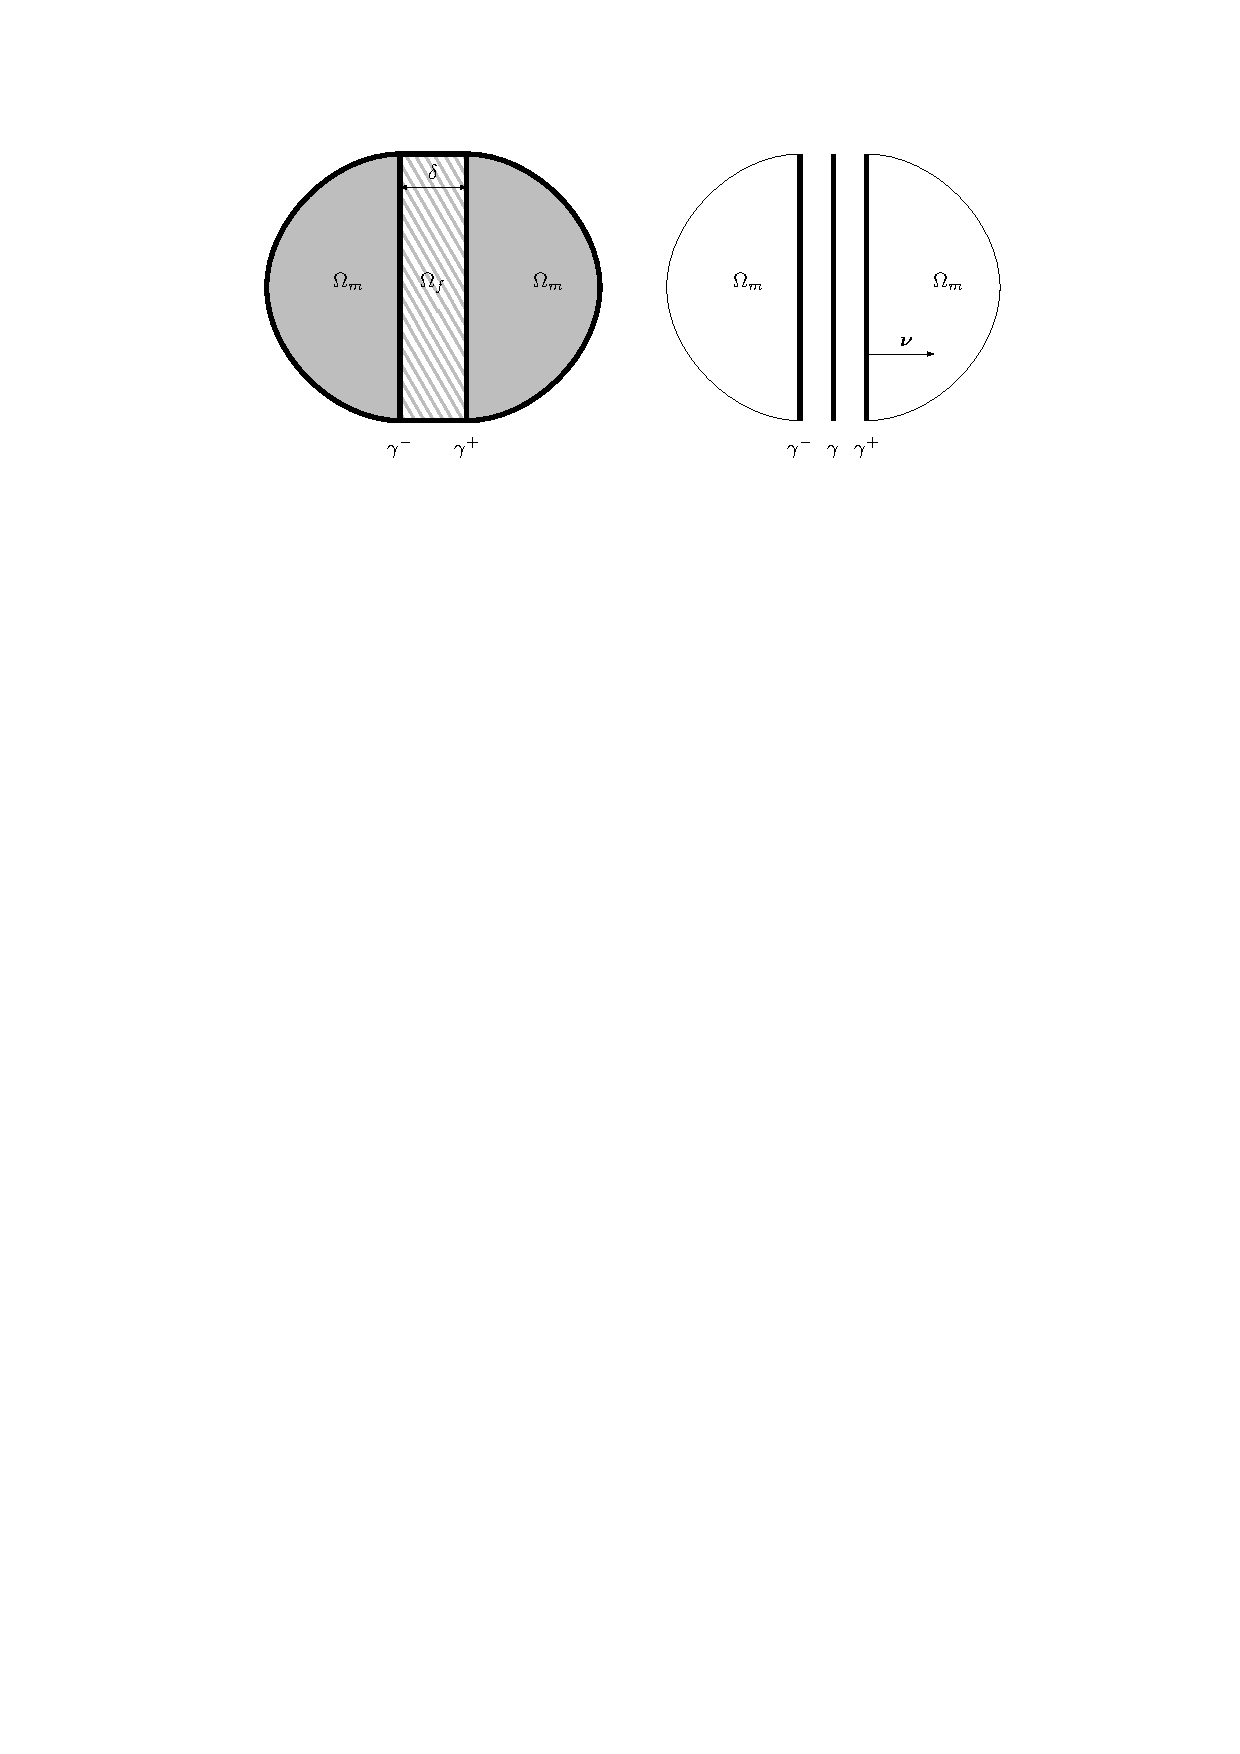
\includegraphics[width=\textwidth]{figures/omegas}
\caption{The domain of the full model (left) and the reduced geometry (right).}
\label{fig:omegas}
\end{figure}

Let $\Omega$ be a bounded, simply connected domain in the Euclidean space $\Real^d$, $d\in\{2,3\}$, with Lipschitz boundary $\partial\Omega$.
We assume that $\Omega$ is composed of two subdomains: the fracture $\Omega_f$ and the matrix $\Omega_m:=\Omega\setminus\overline\Omega_f$.
The matrix is assumed to be divided into two parts (see Figure \ref{fig:omegas}).
For simplicity we consider straight fracture, i.e. there is a subset $\gamma$ of a hyperplane in $\Real^d$ and a number $\delta>0$ so that
\eq{ \Omega_f = \{\xx+s\nnu;~\xx\in\gamma,~s\in(-\tfrac\delta2,\tfrac\delta2)\}, }
where $\nnu$ stands for the unit normal vector to $\gamma$.
The parameter $\delta$ is usually called the aperture or the width of the fracture.

Without loss of generality we can take $\gamma:=\Omega\cap\left(\{0\}\times\Real^{d-1}\right)$ and $\nnu:=(1,0,0)^\top$.
Then the two parts of $\Omega_m$ are interacting with $\Omega_f$ via the interfaces
\eq{ \gamma^+:=\Omega\cap\big( \{\tfrac\delta2\}\times \Real^{d-1}\big), \quad \gamma^-:=\Omega\cap\big( \{ -\tfrac\delta2\}\times \Real^{d-1}\big). }
The symbol $\prtl\gamma$ shall denote the relative boundary of $\gamma$.

% We shall derive a model of poroelasticity on the reduced geometry consisting of $\Omega_m$ and $\gamma$.
The basic hydro-mechanical interaction in a porous media is described by the Biot system of poroelasticity.
In context of this paper it reads:
\begin{subequations}
\label{eq:biot}
\begin{align}
    \label{eq:lin_el}
    -\div \bbsigma + \nabla(\alpha p) &= \ff &&\mbox{ in }\Omega_m\cup\Omega_f,\\
\label{eq:biot_darcy}    \prtl_t\left(Sp + \div(\alpha\uu)\right) + \div\qq &= g &&\mbox{ in }\Omega_m\cup\Omega_f,
\end{align}
\end{subequations}
Here, the displacement $\uu$ and the pressure $p$ are the principal unknowns; further $\alpha$ is the Biot effective stress parameter, $\ff$ the body force, $S$ the storativity, $g$ the fluid source.
The stress tensor $\bbsigma$ is given by the Hooke law:
\eq{ \bbsigma = \tn C\nabla\uu, }
where $\tn C$ is the $4^{\rm th}$-order elasticity tensor, and the flux $\qq$ is given by the Darcy law:
\eq{ \quad \qq = -\tn K\nabla p }
via the hydraulic conductivity tensor $\tn K$.
To complete the equations in $\Omega$, we require that
\eq{ \label{eq:continuity_on_gamma_pm} p,\uu,\qq\cdot\nnu,\bbsigma\nnu \mbox{ are continuous on } \gamma^\pm. }

In what follows, we shall assume that the physical parameters $\alpha,S,\tn C,\tn K$ are constant in $\Omega_m$, $\Omega_f$, respectively.
To distinguish values in $\Omega_m$ and $\Omega_f$, we shall use the subscripts ``$m$'' and ``$f$'', i.e. $\alpha_m := \alpha_{|\Omega_m}$, $\alpha_f := \alpha_{|\Omega_f}$ etc.
In addition, it is assumed that $\tn C_*$ and $\tn K_*$, $*\in\{m,f\}$, have the usual symmetries:
\eq{ \label{eq:sym_C} \forall \tn A,\tn B\in\Real^{d\times d}:~ \tn C_*\tn A:\tn B=\tn C_*\tn A^\top:\tn B=\tn C_*\tn A:\tn B^\top=\tn C_*\tn B:\tn A, }
\eq{ \tn K_* = \tn K_*^\top, }
and are positive definite:
\eq{ \label{eq:pos_def_C} \forall\tn A\in\Real^{d\times d}_{sym}:~\tn C_*\tn A:\tn A \ge C_1|\tn A|^2, }
\eq{ \forall\vv\in\Real^d:~\tn K_*\vv\cdot\vv \ge C_2|\vv|^2,\quad *\in\{m,f\}. }
Here $\Real^{d\times d}_{sym}$ stands for the set of symmetric $d\times d$ matrices and $|\tn A|$ denotes the Frobenius norm, i.e. $|\tn A|^2=\tn A:\tn A$.
It is not difficult to observe that \eqref{eq:sym_C} and \eqref{eq:pos_def_C} imply:
\eq{ \label{eq:pos_def_C_gen} \forall\tn A\in\Real^{d\times d}:~\tn C_*\tn A:\tn A \ge C_1\left|\frac{\tn A+\tn A^\top}2\right|^2. }
A further natural requirement is that $\nnu$ is an eigenvector of $\tn K_f$, i.e.
\eq{\label{eq:normal_conductivity} \tn K_f\nnu = k_f\nnu, }
where $k_f>0$ is the hydraulic conductivity in orthogonal direction to $\gamma$.




\section{Tangential and normal calculus in fracture}\label{sec:calculus}

Let $\tn P := \nnu\otimes\nnu$ be the orthogonal projector to $\gamma$.
For any $\vv\in\Real^d$ and $\tn A\in\Real^{d\times d}$ we shall define the orthogonal decomposition into normal and tangential direction to $\gamma$:
\eq{ \vv = \tn P\vv + (\tn I-\tn P)\vv =:\vv_\nu + \vv_\tau, }
\eq{ \tn A = \tn A\tn P + \tn A(\tn I-\tn P) =: \tn A_\nu + \tn A_\tau. }
Likewise we decompose differential operators acting on vector- and tensor-valued functions:
\eq{ \label{eq:grad_sc} \nabla f = (\nabla f)_\nu + (\nabla f)_\tau =: \nabla_\nu f + \nabla_\tau f, }
\eq{ \label{eq:grad_vc} \nabla\vv = (\nabla\vv)_\nu + (\nabla\vv)_\tau =: \nabla_\nu\vv + \nabla_\tau\vv, }
\eq{ \div\vv = \div\vv_\nu + \div\vv_\tau =: \div_\nu\vv + \div_\tau\vv, }
\eq{ \label{eq:div_tn} \div\tn A = \div(\tn P\tn A) + \div((\tn I-\tn P)\tn A) =: \div_\nu\tn A + \div_\tau\tn A. }
Let $w$ be a function defined in $\gamma^+$ and $\gamma^-$.
Shifting its argument to $\gamma$, we obtain new functions
\eq{ w^{\opm}(\xx) := w(\xx\pm\tfrac\delta2\nnu), ~\xx\in\gamma. }
Now we can introduce the average and the jump operator:
\eq{ \avg{w} := \frac{w^\oplus+w^\ominus}2,\quad \jmp{w} := w^\oplus-w^\ominus. }
When integrating across the fracture, we shall write
\[ \int w\dn := \int w(\cdot+s\nnu)\d s. \]
The symbol $\overline w$ will denote the integral mean of $w$ across the fracture aperture, i.e.
\eq{\label{eq:def_mean} \overline w(\xx):=\frac1\delta\int_{-\tfrac\delta2}^{\tfrac\delta2} w(\xx) \dn,~\xx\in\gamma. }
Then, for all sufficiently smooth functions $f$, $\vv$ and $\tn A$ defined in $\Omega_f$ it holds:
\eq{ \label{eq:int_grad_nu_sc}
\int_{-\tfrac\delta2}^{\tfrac\delta2}\nabla_\nu f\dn = \int_{-\tfrac\delta2}^{\tfrac\delta2}\nnu\frac{\rm d}{{\rm d}s}\left(f(\cdot+s\nnu)\right)\d s = \jmp{f}\nnu,
}
\eq{ \label{eq:div_nu_vc}
\int_{-\tfrac\delta2}^{\tfrac\delta2}\div_\nu\vv\dn = \int_{-\tfrac\delta2}^{\tfrac\delta2}\nnu\cdot\frac{\rm d}{{\rm d}s}\left(\vv(\cdot+s\nnu)\right)\d s = \jmp{\vv}\cdot\nnu,
}
\eq{ \label{eq:int_grad_nu_vc} \int_{-\tfrac\delta2}^{\tfrac\delta2}\nabla_\nu\vv\dn = \jmp{\vv}\otimes\nnu, }
\eq{ \label{eq:int_div_nu_tn} \int_{-\tfrac\delta2}^{\tfrac\delta2}\div_\nu\tn A \dn = \jmp{\tn A^\top}\nnu. }
We also have the Green identity in $\gamma$:
\eq{ \int_\gamma(\div_\tau\vv)w = \int_{\prtl\gamma}(\vv\cdot\nn)w - \int_\gamma\vv\cdot\nabla_\tau w, }
where $\nn$ denotes the unit outward normal to $\partial\gamma$.



\section{Dimension reduction}

Let us assume that $(\uu,p)$ is a smooth solution of \eqref{eq:biot}--\eqref{eq:continuity_on_gamma_pm}.
Our aim is to obtain appropriate equations that are satisfied by the averages $(\ubar,\pbar)$ in $\gamma$.


\subsection{Continuum-fracture model for elasticity}\label{sec:reduction_elasticity}

Integrating \eqref{eq:lin_el} over the fracture aperture and decomposing the differential operators yields:
\eq{\label{eq:lin_el_int} \int_{-\tfrac\delta2}^{\tfrac\delta2}\left(-\div_\nu\bbsigma + \nabla_\nu(\alpha p)\right)\dn + \int_{-\tfrac\delta2}^{\tfrac\delta2}\left(-\div_\tau\bbsigma + \nabla_\tau(\alpha p)\right)\dn = \delta\overline\ff. }
The first term on the left hand side of \eqref{eq:lin_el_int} can be rewritten using the formulae \eqref{eq:int_grad_nu_sc} and \eqref{eq:int_div_nu_tn}:
\eq{\label{eq:decomp_el_nu} \int_{-\tfrac\delta2}^{\tfrac\delta2}\left(-\div_\nu\bbsigma + \nabla_\nu(\alpha p)\right)\dn = -\jmp\bbsigma\nnu + \alpha_f\jmp p\nnu. }
For the second term we use the definition of $\bbsigma$ and the fact that the integral over fracture aperture commutes with tangential gradient:
\eq{\label{eq:decomp_el_tau} \int_{-\tfrac\delta2}^{\tfrac\delta2}\left(-\div_\tau\bbsigma + \nabla_\tau(\alpha p)\right)\dn = -\delta\div_\tau\tn C_f\overline{\nabla\uu} + \delta\nabla_\tau(\alpha_f\pbar). }
% 
% \eq{\label{eq:decomp_div_sigma}
% \int_{-\tfrac\delta2}^{\tfrac\delta2}\div\bbsigma\dn = \int_{-\tfrac\delta2}^{\tfrac\delta2}\left(\div_\tau\bbsigma + \div_\nu\bbsigma\right) \dn
% = \delta\div_\tau\tn C_f\overline{\nabla\uu} + \jmp{\bbsigma}\nnu,
% }
% \eq{\label{eq:decomp_grad_alpha_p} \int_{-\tfrac\delta2}^{\tfrac\delta2}\nabla(\alpha p)\dn = \int_{-\tfrac\delta2}^{\tfrac\delta2} \left(\nabla_\tau(\alpha p) + \nabla_\nu(\alpha p)\right) \dn
% = \delta\nabla_\tau(\alpha_f\pbar) + \alpha_f\jmp{p}\nnu.
% }
The averaged gradient can be expressed using \eqref{eq:int_grad_nu_vc} as follows:
\eq{\label{eq:avg_grad_u} \overline{\nabla\uu} = \nabla_\tau\ubar + \jmp{\uu}\otimes\tfrac{\nnu}\delta. }
Now we turn to approximation of the normal stress $\bbsigma\nnu$ on $\gamma^\pm$.
Using one-sided difference quotients, we can define the approximate normal gradient of $u$ in the positive/negative half of the fracture:
\eq{ \agrad_\nu^\opm[\uu,\ubar] := \pm\frac2\delta(\uu^\opm-\ubar)\otimes\nnu \approx (\nabla_\nu\uu)^\opm. }
For the tangential gradient we shall use the approximation
\eq{ (\nabla_\tau\uu)^\opm \approx \nabla_\tau\ubar. }
Hence the approximate one-sided gradient reads:
\eq{ \agrad^\opm[\uu,\ubar]:=\nabla_\tau\ubar + \agrad_\nu^\opm[\uu,\ubar]. }
We can observe that the approximate gradients satisfy
\eq{ \overline{\nabla\uu} = \avg{\agrad[\uu,\ubar]}. }
Then the approximate normal stress on $\gamma^\pm$ is given by
\eq{\label{eq:def_T} \tt^\opm[\uu,\ubar] := \left(\tn C_f\agrad^\opm[\uu,\ubar]\right)\nnu, }
so that $\bbsigma^\opm\nnu \approx \tt^\opm$.
Collecting \eqref{eq:lin_el_int}--\eqref{eq:avg_grad_u} and \eqref{eq:def_T} and neglecting the approximation error, we obtain the averaged counterpart of \eqref{eq:lin_el}:
\eq{ \label{eq:lin_el_frac} -\delta\div_\tau\left(\tn C_f\avg{\agrad[\uu,\ubar]}\right) + \delta\nabla_\tau(\alpha_f\pbar) - \jmp{\tt[\uu,\ubar]} + \alpha_f\jmp{p}\nnu = \delta\overline\ff. }
The continuity of $\bbsigma\nnu$ on $\gamma^\pm$ is approximated by the condition
\eq{ \label{eq:interface_el} (\tn C_m\nabla\uu_{|\Omega_m})\nnu = \tt^\opm[\uu,\ubar] \mbox{ on }\gamma^\pm. }









\subsection{Continuum-fracture model for flow}\label{sec:reduction_flow}

Let us integrate \eqref{eq:biot_darcy} over the fracture aperture.
We get:
\eq{ \label{eq:darcy_int} \prtl_t\left(\delta S\pbar + \int_{-\tfrac\delta2}^{\tfrac\delta2}\div(\alpha\uu)\dn\right) + \int_{-\tfrac\delta2}^{\tfrac\delta2}\div\qq\dn = \delta\overline g. }
The first integral in \eqref{eq:darcy_int} will be rewritten using \eqref{eq:div_nu_vc}:
\ml{ \label{eq:div_alpha_u_int} \int_{-\tfrac\delta2}^{\tfrac\delta2}\div(\alpha\uu)\dn = \int_{-\tfrac\delta2}^{\tfrac\delta2}\left(\div_\tau(\alpha_f\uu_f) + \div_\nu(\alpha\uu)\right)\dn\\
= \delta\div_\tau(\alpha_f\ubar) + \alpha_f\jmp{\uu}\cdot\nnu. }
Similarly we obtain:
\eq{ \label{eq:div_q_int} \int_{-\tfrac\delta2}^{\tfrac\delta2}\div\qq = \int_{-\tfrac\delta2}^{\tfrac\delta2}\left(\div_\tau\qq + \div_\nu\qq\right) 
= \delta\div_\tau(\tn K_f\overline{\nabla p}) + \jmp\qq\cdot\nnu, }
where
\eq{ \overline{\nabla p} = \nabla_\tau\pbar + \frac1\delta\jmp{p}\nnu. }
From the definition of $\div_\tau$ and \eqref{eq:normal_conductivity} it then follows that
\eq{ \label{eq:div_tau_K_gp} \div_\tau(\tn K_f\overline{\nabla p}) = \div_\tau(\tn K_f\nabla_\tau\pbar). }
To express the approximation of the normal flux $\qq\cdot\nnu$ on $\gamma^\pm$ we use the approximation
\eq{ \label{eq:approx_p} (\nabla_\nu p)^\opm \approx \frac{\pm(p^\opm-\pbar)}{\tfrac\delta2}\nnu. }
% provided that $\nabla^2 p$ is bounded in $\Omega_f$.
Using this, we can write:
\eq{ \label{eq:approx_flux} -\qq^\opm\cdot\nnu = \tn K_f\nabla p^\opm\cdot\nnu = k_f(\nabla_\nu p)^\opm\cdot\nnu \approx \pphi^\opm, }
where the approximate normal fluxes $\pphi^\opm$ are given by
\eq{ \label{eq:def_F} \pphi^\opm = \pphi^\opm[p,\pbar] := \pm k_f\frac2\delta(p^\opm-\pbar). }
% 
Neglecting the approximation error, we obtain from \eqref{eq:darcy_int}--\eqref{eq:def_F} the averaged flow equation:
\eq{ \label{eq:flow_frac} \delta\prtl_t\left(S_f\pbar + \div_\tau(\alpha_f\ubar)\right) -\delta\div_\tau(\tn K_f\nabla_\tau\pbar) +\alpha_f\jmp{\prtl_t\uu}\cdot\nnu - \jmp \pphi = \delta\overline g. }
Continuity of flux through $\gamma^\pm$ is approximated by the condition
\eq{ \label{eq:interface_flow} \tn K_m\nabla p_{|\Omega_m}\cdot\nnu = \pphi^\opm \mbox{ on }\gamma^\pm. }




\section{Well-posedness of mixed-dimensional linear elasticity}\label{sec:wellposedness_elasticity}

In this section we consider only the mechanical part of the problem.
Let $\Gamma:=\prtl\Omega_m\cap\prtl\Omega$, $H^1_0(\gamma;\Real^d)$ denote the Sobolev space of vector-valued functions in $\gamma$ with zero traces on $\prtl\gamma$ and $H^1_\Gamma(\Omega_m;\Real^d)$ the Sobolev space of vector-valued functions in $\Omega_m$ vanishing on $\Gamma$.

Given loads $\ff:\Omega_m\to\Real^d$, $\FF:\gamma\to\Real^d$, we want to find the displacement fields $\uu:\Omega_m\to\Real^d$ and $\U:\gamma\to\Real^d$ satisfying the following boundary-value problem:
\begin{subequations}\label{eq:lin_el_problem}
\begin{align}
-\div(\tn C_m\nabla\uu) &= \ff &&\mbox{in }\Omega_m,\\
-\delta\div_\tau\left(\tn C_f\avg{\agrad[\uu,\U]} \right) - \jmp{\tt[\uu,\U]} &= \FF &&\mbox{in }\gamma,\\
(\tn C_m\nabla\uu)\nnu &= \tt^\opm[\uu,\U] &&\mbox{on }\gamma^\pm,\\
\uu &=\vc0&&\mbox{on }\Gamma,\\
\U &=\vc 0&&\mbox{on }\prtl\gamma.
\end{align}
\end{subequations}

\subsection{Weak formulation}
The weak formulation of \eqref{eq:lin_el_problem} is derived by multiplying the equations in $\Omega_m$ and $\gamma$ by suitable test functions $\vv$, $\V$, respectively, integrating by parts and applying the boundary and interface conditions.
After that we arrive at the identity
\ml{ \int_{\Omega_m}\tn C_m\nabla\uu:\nabla\vv
 + \delta\int_\gamma\tn C_f\avg{\agrad[\uu,\U]}:\nabla_\tau\V\\
 + \int_\gamma\left(\jmp{\tt[\uu,\U]\cdot(\vv-\V)}\right)
 = \int_{\Omega_m}\ff\cdot\vv + \int_\gamma\FF\cdot\V. }
From the definition of $\tt^\opm$ and $\agrad_\nu^\opm$ it follows that
\eq{ \tt^\opm[\uu,\U]\cdot(\vv^\opm-\V) %= \tn C_f(\nabla_\tau\V+\agrad_\nu^\opm[\vv,\V]):(\vv^\opm-\V)\otimes\nnu\\
= \pm\frac\delta2\tn C_f\agrad^\opm[\uu,\U]:\agrad_\nu^\opm[\vv,\V], }
hence
\eq{ \jmp{\tt[\uu,\U]\cdot(\vv-\V)} = \delta\avg{\tn C_f\agrad[\uu,\U]:\agrad_\nu[\vv,\V]}, }
and so the resulting identity reads:
\eq{ \int_{\Omega_m}\tn C_m\nabla\uu:\nabla\vv
 + \delta\int_\gamma\avg{\tn C_f\agrad[\uu,\U]:\agrad[\vv,\V]}
  = \int_{\Omega_m}\ff\cdot\vv + \int_\gamma\FF\cdot\V. }
% 
Let us define the space
\eq{ \Vel :=H^1_\Gamma(\Omega_m;\Real^d)\times H^1_0(\gamma;\Real^d) }
equipped by the norm $\norm{(\vv,\vc V)}_\Vel := (\norm{\nabla\vv}_{L^2(\Omega)}^2 + \norm{\nabla_\tau\vc V}_{L^2(\gamma)}^2)^{1/2}$ and the forms
\eq{ a((\uu,\U), (\vv,\vc V)) := \int_{\Omega_m}\tn C_m\nabla\uu:\nabla\vv
 + \delta\int_\gamma\avg{\tn C_f\agrad[\uu,\U]:\agrad[\vv,\V]}, }
\eq{ l((\vv,\vc V)) := \dual{(\ff,\FF)}{(\vv,\V)}_\Vel = \dual{\ff}{\vv}_{H^1_\Gamma(\Omega_m;\Real^d)} + \dual{\FF}{\V}_{H^1_0(\gamma;\Real^d)}. }
Then the weak formulation of \eqref{eq:lin_el_problem} reads:
\eq{ \label{eq:el_weak} \left.\begin{minipage}{0.7\textwidth}
Find $(\uu,\U)\in \Vel$ such that
\[ \forall(\vv,\vc V)\in \Vel:~a((\uu,\U),(\vv,\vc V)) = l((\vv,\vc V)). \]
\end{minipage}\right\} }

\subsection{Korn type inequalities}
Before establishing the well-posedness of \eqref{eq:el_weak} we prove a suitable Korn type inequality.
For any function $\V\in H^1(\gamma;\Real^d)$ we denote its symmetrized tangential gradient by
\eq{ \ep_\tau\V := \frac12(\nabla_\tau\V + (\nabla_\tau\V)^\top). }
Similarly for a pair of functions $(\vv,\V)\in\Vel$ we define its symmetrized approximate gradient by
\eq{ \aep^\opm[\vv,\V] := \frac12(\agrad^\opm[\vv,\V]+(\agrad^\opm[\vv,\V])^\top). }
% Similarly, for a pair $(\vv,\V)\in\Vel$ we define the symmetrized approximate normal gradient
% \eq{ \ep_\nu^\opm[\vv,\V] := \frac12\left(\agrad_\nu^\opm[\vv,\V]+(\agrad_\nu^\opm[\vv,\V])^\top\right). }
We have the following Korn inequality in $H^1_0(\gamma)$.
% 
\begin{lemma}\label{th:korn_tau}
There exists a constant $C_3>0$ such that for all $\V\in H^1_0(\gamma;\Real^d)$ it holds:
\eq{ \label{eq:korn_tau} \norm{\ep_\tau\V}_{L^2(\gamma)}^2 \ge C_3\norm{\nabla_\tau\V}_{L^2(\gamma)}^2. }
\end{lemma}
% 
\begin{proof}
Let $\V\in H^1_0(\gamma;\Real^d)$.
Then, by mapping $\V$ isometrically from $\gamma$ to a subset of $\Real^{d-1}$, we apply the Korn inequality to the tangential part $\V_\tau$, which implies
\eq{ \norm{\ep_\tau\V_\tau}_{L^2(\gamma)}^2 \ge C_K\norm{\nabla_\tau\V_\tau}_{L^2(\gamma)}^2. }
From the definition of tangential and normal operators it follows that
% \eq{ |\ep_\tau\V|^2 = |\ep_\tau\V_\tau|^2 + \tfrac12|\nabla_\tau\V_\nu|^2, }
% so that
\ml{ \norm{\ep_\tau\V}_{L^2(\gamma)}^2 = \norm{\ep_\tau\V_\tau}_{L^2(\gamma)}^2 + \tfrac12\norm{\nabla_\tau\V_\nu}_{L^2(\gamma)}^2\\
% \ge C_K\norm{\nabla_\tau\V_\tau}_{L^2(\gamma)}^2 + \tfrac12\norm{\nabla_\tau\V_\nu}_{L^2(\gamma)}^2
\ge \min\{C_K,\tfrac12\}\norm{\nabla_\tau\V}_{L^2(\gamma)}^2, }
which proves \eqref{eq:korn_tau}.
\end{proof}

Now we can prove a variant of the Korn inequality which takes into account the approximate gradient in $\gamma$.
\begin{lemma}
There exists a constant $C_4>0$ such that for all $(\vv,\V)\in \Vel$ it holds:
\eq{\label{eq:korn_frac} \norm{\ep\vv}_{L^2(\Omega_m)}^2 + \avg{\norm{\aep[\vv,\V]}_{L^2(\gamma)}^2} \ge C_4\norm{(\vv,\V)}_\Vel^2. }
\end{lemma}
\begin{proof}
Let us assume for contradiction that there is a sequence $\{(\vv_n,\V_n)\}_{n=1}^\infty$ in $\Vel$ such that
\eq{\label{eq:korn_asm_contra} \norm{\ep\vv_n}_{L^2(\Omega_m)}^2 + \avg{\norm{\aep[\vv_n,\V_n]}_{L^2(\gamma)}^2} < \frac1n\norm{(\vv_n,\V_n)}_\Vel^2. }
Without loss of generality we may assume that $\norm{(\vv_n,\V_n)}_\Vel=1$, so that
\eq{\label{eq:korn_weak_vV} (\vv_n,\V_n)\weakly (\vv,\V) \mbox{ weakly in }\Vel, ~n\to\infty, }
where $(\vv,\V)\in \Vel$, passing eventually to a subsequence.
From \eqref{eq:korn_asm_contra} and the Korn inequality in $H^1_\Gamma(\Omega_m;\Real^d)$ it follows that
\eq{\label{eq:korn_strong_v} \vv_n\to\vc 0 \mbox{ strongly in }H^1_\Gamma(\Omega_m;\Real^d),~n\to\infty, }
implying that $\vv=\vc 0$.
From \eqref{eq:korn_asm_contra} it also follows that
\eq{\label{eq:korn_conv_approx_grad} \aep^\opm[\vv_n,\V_n] \to 0 \mbox{ strongly in }L^2(\gamma;\Real^{d\times d}),~n\to\infty. }
Using this together with the definition of $\aep^\opm$, \eqref{eq:korn_weak_vV}, \eqref{eq:korn_strong_v} and the embedding $H^1(\Omega_m)\hookrightarrow L^2(\gamma)$, we obtain:
\eq{ \ep_\tau\V = \pm\frac1\delta(\V\otimes\nnu+\nnu\otimes\V), }
from which it follows that $\V=\vc 0$.
With help of the compact embedding $H^1(\gamma)\hookrightarrow L^2(\gamma)$ we deduce from \eqref{eq:korn_conv_approx_grad} that $\ep_\tau\V_n\to 0$ strongly in $L^2(\gamma;\Real^{d\times d})$, $n\to\infty$.
Lemma \ref{th:korn_tau} then implies that also $\V_n\to\vc 0$ strongly in $H^1_0(\gamma;\Real^d)$, $n\to\infty$.
Finally, having shown the strong convergence of $\{(\vv_n,\V_n)\}_{n=1}^\infty$, we observe that
\eq{ 1 = \lim_{n\to\infty}\norm{(\vv_n,\V_n)}_\Vel = \norm{(\vv,\V)}_\Vel = 0, }
which is a contradiction.
Therefore the proof is finished.
\end{proof}

\subsection{Existence and uniqueness of solutions}
In the following lemma we prove the ellipticity of $a$.
\begin{lemma}
The bilinear form $a$ is bounded and elliptic in $\Vel$.
\end{lemma}
\begin{proof}
The boundedness of $a$ is a consequence of the embedding $H^1(\Omega_m)\hookrightarrow L^2(\gamma)$ and standard inequalities; we prove only the ellipticity.
For any $(\vv,\V)\in \Vel$ we have:
\eq{ \label{eq:a_uu2} a((\vv,\V),(\vv,\V)) = \int_{\Omega_m}\tn C_m\nabla\vv:\nabla\vv
+ \delta\int_\gamma\avg{\tn C_f\agrad[\vv,\V]:\agrad[\vv,\V]}. }
Now we can apply \eqref{eq:pos_def_C_gen} and \eqref{eq:korn_frac}, which yields:
\ml{ a((\vv,\V),(\vv,\V)) \ge C_1\norm{\ep\vv}_{L^2(\Omega_m)}^2 + C_1\delta\avg{\norm{\aep[\vv,\V]}_{L^2(\gamma)}^2}\\
\ge C_1 C_4\min\{1,\delta\}\norm{(\vv,\V)}_\Vel^2. }
From this we see that $a$ is elliptic with the constant $C_1 C_4\min\{1,\delta\}$.
\end{proof}

It is not difficult to show that $l$ is bounded in $\Vel$ under appropriate assumptions about $\ff$ and $\FF$.
Hence we have the following result as a direct consequence of the Lax-Milgram theorem.

\begin{theorem}
Let $(\ff,\FF)\in\Vel^*$. Then problem \eqref{eq:el_weak} has a unique solution which satisfies:
\eq{ \norm{(\uu,\U)}_\Vel \le \frac{\norm{(\ff,\FF)}_{\Vel^*}}{C_1 C_4\min\{1,\delta\}}. }
\end{theorem}

Let us now consider the time-dependent case.
Given a pair of functions $(\ff,\FF):(0,T)\to\Vel^*$ defined in the interval $(0,T)$, we denote by $(\uu(t),\U(t))$ the solution of \eqref{eq:el_weak} with the data $(\ff(t),\FF(t))$, $t\in(0,T)$.
We obtain:

\begin{corollary}
Let $(\ff,\FF)\in C([0,T];\Vel^*)$. Then $(\uu,\U)\in C([0,T];\Vel)$.
If in addition $(\dt\ff,\dt\FF)\in L^2(0,T;\Vel^*)$, then $(\dt\uu,\dt\U)\in L^2(0,T;\Vel)$.
\end{corollary}










% \section{Mixed formulation for incompressible elastic material}
% TOHLE JE ZATIM JEN PRO ROVINNE PUKLINY
% 
% In this section we shall assume that the elasticity tensor has the form
% \[ c_{ijkl} = \mu(\delta_{ik}\delta_{jl} + \delta_{il}\delta_{jk}) + \lambda\delta_{ij}\delta_{kl}, ~i,j,k,l=1,...,d, \]
% and hence
% \[ \vc\sigma[\uu,p] = 2\mu\ep[\uu] + (\lambda\div\uu - \alpha p)\tn I. \]
% Further we shall assume that the material parameter $\alpha$ is constant in $\Omega_{mi}$, $i=1,2$ and in $\gamma$.
% We aim to derive a formulation which is suitable for the incompressible case, i.e. when $\lambda\to\infty$.
% For this reason we introduce a new quantity
% \[ \phi:=\alpha p-\lambda\div\uu, \]
% so that the stress tensor becomes
% \[ \vc\sigma=\vc\sigma[\uu,\phi] = 2\mu\ep[\uu] - \phi\tn I. \]
% The Biot system in the matrix domain now reads:
% \[ \left.\begin{aligned}
% -\div(2\mu\ep[\uu_i]) + \nabla\phi_i &= \ff\\
% \prtl_t\left(\left(\frac1M+\frac{\alpha^2}\lambda\right)p_i - \frac\alpha\lambda\phi_i\right)-\div(\tn K\nabla p_i) &= g\\
% \div\uu_i - \frac\alpha\lambda p_i + \frac1\lambda\phi_i &= 0
% \end{aligned}\right\} \mbox{ in }\Omega_{mi}, ~i=1,2. \]
% After integrating across the fracture we obtain:
% % The continuum-fracture system for poroelasticity now reads:
% \[ \left.\begin{aligned}
% -\div_\tau(2\delta\mu\ep_\tau[\uu_f]) + \nabla_\tau(\delta\phi_f) + \sum_{i=1}^2\tilde{\vc Q}_i + \tilde{\vc R} &= \delta\overline\ff\\
% \prtl_t\left(\delta\left(\frac1M+\frac{\alpha^2}\lambda\right) p_f - \delta\frac\alpha\lambda\phi_f\right)-\div_\tau(\delta\tn K\nabla_\tau p_f)  + \sum_{i=1}^2F_i &= \delta \overline g\\
% \div_\tau(\delta\uu_f) + \sum_{i=1}^2(\uu_f-\uu_i)\cdot\nn_i - \delta\frac\alpha\lambda p_f + \frac\delta\lambda\phi_f &= 0
% \end{aligned} \right\} \mbox{ in }\gamma, \]
% with the interface conditions
% \[ \left.\begin{aligned}
% \vc\sigma[\uu_i,\phi_i]\nn_i &= \tilde{\vc Q}_i \\
% \tn K\nabla p_i\nn_i &= F_i \end{aligned} \right\} \mbox{ on }\gamma_i,~i=1,2, \]
% where
% \[ \begin{aligned}
% \tilde{\vc Q}_i &= 2\mu\ep_\tau[\uu_f]\nn_i + \frac4\delta\mu(\uu_f-\uu_i) - \phi_f\nn_i, \\
% \tilde{\vc R} &= \sum_{i=1}^2\div_\tau(\mu(\uu_i\otimes\nn_i+\nn_i\otimes\uu_i)). \end{aligned} \]
% One can notice that in the limit $\lambda\to\infty$, the flow and elasticity become independent.



\bibliographystyle{abbrvnat}
\bibliography{flow123d_doc.bib}
%%%%%%%%%%%%%%%%%%%%%%%%%%%%%%%%%%%%%%%%%%%%%%%%%%%%%%%%%%%%%%%%%%%%%%%%%%%%%%%%%%%%%%%%%%%%%%%%%%%%%%%%%%%%%%%%%


\end{document}


